\documentclass[mastersproject,12pt]{wuthesis}     %% LaTeX2e document.
%
% Use one of the following
% \documentclass[mastersthesis,12pt]{wuthesis}
% \documentclass[dscthesis,12pt]{wuthesis}
% \documentclass[phdthesis,12pt]{wuthesis}
%
% If you want to use other packages such as amstex, or epsfig
% \usepackage them here.
%
% epsfig, ellipsis, and caption are 'packages' for LaTeX2e and
% should be part of your distribution.  If not talk to your
% sysadmin
\usepackage{epsfig}
\usepackage{ellipsis}
\usepackage[center]{caption}
%%%%%%%%%%%%%%%%%%%%%%%%%%%%%%%%%%%%%%%%%%%%%%%%%%%%%%%%%%%%%%%%%%%%%%%%%%%%%
%%
%% These commands customize the `wuthesis' package for me
%%
%%%%%%%%%%%%%%%%%%%%%%%%%%%%%%%%%%%%%%%%%%%%%%%%%%%%%%%%%%%%%%%%%%%%%%%%%%%%%

%% Enter your official name
\renewcommand{\thesisauthor}{David Ross}
\renewcommand{\thesisauthorlastname}{Ross}

%% Enter your previous degrees
%% If you have no previous degrees remember to remove the comma too.
%\renewcommand{\thesisauthorpreviousdegrees}{, J.D.}

%% Enter department name
\renewcommand{\thesisdepartment}{Department of Computer Science and Engineering}
\renewcommand{\thesisfield}{Computer Science}

%% Enter date of graduation
\renewcommand{\thesismonth}{May}
\renewcommand{\thesisyear}{2009}

%% Enter title of thesis
\renewcommand{\thesistitle}{A Mock Thesis on the Proper Formatting of Theses and Dissertations for Engineering-Based Grad Students}
\renewcommand{\thesisshorttitle}{The Proper Format of Theses}

%% Enter the copyright holder ( DEFAULT is \thesisauthor )
%\renewcommand{\thesiscopyrightholder}{\thesisauthor}

%% Enter supervisor name
\renewcommand{\thesissupervisor}{Professor Robert Pless}
\renewcommand{\thesiscommittee}{Tao Ju \\
	Robert Pless \\
	Bill Smart}

%% Enter the dedication
\renewcommand{\thesisdedication}{Dedicated to my parents.}

%%%%%%%%%%%%%%%%%%%%%%%%%%%%%%%%%%%%%%%%%%%%%%%%%%%%%%%%%%%%%%%%%%%%%%%%%%%%%
%%
%% This paper is construced from other files.  Each \include'd file
%% begins a chapter.  This is done for easy developement and revision.
%%
%%%%%%%%%%%%%%%%%%%%%%%%%%%%%%%%%%%%%%%%%%%%%%%%%%%%%%%%%%%%%%%%%%%%%%%%%%%%%

\begin{document}

\frontmatter
%%
%  This is all that frontmatter stuff
%
%  This way I can 'not' include it easily

% NOTE: do not put any text in the thesistitlepage, thesiscopyrightpage,
% or thesisdedicationpage sections.  If you want to use these pages, then you
% should remove the notes below (e.g., by uncommenting the \iffalse
% and \fi lines) and change the appropriate fields in thesis-main.tex.
% This will ensure that the copyright and dedication lines are positioned
% and formatted correctly.  Additionally, remove the
% thesisacknowledgmentpostscript and listoftablespostscript sections, since
% these are used to add explanatory notes which shouldn't be there in normal
% theses.

\begin{thesistitlepage}               %% Generate the title page.
%\iffalse
\begin{singlespace}
\tiny
{\small \textbf{How to use this document:}}
This sample document outlines guidelines for the proper formatting of theses
and dissertations for Master's and D.Sc.\ degree seeking students within the
School of Engineering at Washington University.  (Ph.D.\ students can also make
use of this document; see special note below.)  This document is formatted
using the same guidelines which it describes.  Consequently, by making an extra
copy of this document you can use it as a template into which you can insert
your own thesis or dissertation textual matter, replacing the original text
with your own while still retaining the general formatting contained within.
This document/template can be downloaded (as either a Microsoft WORD document
OR as a set of \LaTeX{} files) from the Engineering Student Services' web site
and is located with other engineering graduate forms and guides.

{\small \textbf{Important reminders of what needs to be updated:}}
Be certain to use your own full name wherever appropriate.  After removing
these comments, be sure to vertically center the information on this title page
to assure an equal amount of ``white space'' exists both above and below your
title page information.  Your examination committee will likely contain only
three members if you are a Master�s student, as shown in the sample above.
However, D.Sc.\ committees will typically have five members, and Ph.D.\
committees will have six.  Make sure you use the month and year your degree is
officially to be \uline{earned} on the title page, abstract page, and on any
vita page included.  \uline{If this is for your doctoral degree (i.e., either
D.Sc.\ or Ph.D.),} be sure to change all occurrences of the word ``thesis'' to
display as ``dissertation'', and change ``MASTER OF SCIENCE'' to ``DOCTOR OF
SCIENCE'' or ``DOCTOR OF PHILOSOPHY'', whichever applies.   \uline{IMPORTANT:
If you are a Ph.D.\ student,} you must also change the line above (near the
midsection of this page) to ``A dissertation presented to the Graduate School
of Arts and Sciences'' (but do NOT change the reference to the ``School of
Engineering'' which is at the very top of this page, as that must be left
exactly as shown.

{\small \textbf{Note for Ph.D.\ Students:}}
The formatting contained within this sample document can serve well in
emulating the basic formatting needed for the Ph.D.\ dissertation.   However,
please remember that all Ph.D.\ students are ultimately responsible for meeting
the Graduate School of Arts \& Sciences' formatting guidelines.  The GSAS
dissertation guidelines are published on the Graduate School web site located
with other documentation for GSAS policies and guides.  Be sure to read
``Important reminders'' in paragraph above.
\end{singlespace}
%\fi
\end{thesistitlepage}

\begin{thesiscopyrightpage}                 %% Generate the copyright page.
%\iffalse
\begin{singlespace}
\scriptsize
{\small \textbf{Important Notes Regarding Copyright Option:}} \\
Technically, a thesis or dissertation is protected to some degree by copyright
laws with or without a student having to register his or her claim to
copyright.  However, including a copyright page and applying for registration
of ones claim to copyright provide extra measures of legal protection from
potential copyright infringement.  There is a fee connected with explicitly
registering to copyright ones work; because of this, many students do not
choose to register to copyright their work.  Students should check with their
advisor(s) and/or seek legal advice to gather further information helpful to
making a decision with regards to registering their claim to copyright.  If you
are \uline{not} going to register to copyright your work, then you can choose
to remove this page from your document.  However, if you do choose to
explicitly copyright your work, then leave this page in, change the name to
your name, change the year to the appropriate year in which your degree will be
earned, and remove these notes of informational text.  If a student wishes to
officially ``register'' this claim to copyright, then Masters students will
need to pursue that effort on their own and can find appropriate options by
searching the web; Doctoral students can complete an authorization to apply for
registration (i.e., of their claim to copyright the dissertation) by indicating
this interest in the appropriate area of the UMI Dissertation Publishing
Agreement Form (i.e., on the form which they will submit along with their final
dissertation material) available from the Engineering Student Services web
site.

{\small \textbf{Important Notes Regarding Page Numbering and Margins:}} \\
If you decide to include this copyright page in your final document, do
\uline{not} count the page among your counted pages, and do \uline{not} display
any page number on the page.  \uline{Every sheet of paper in the manuscript
should be numbered except for two:  the title page and this optional copyright
page.}Specifically, the front textual information (which comes before your main
thesis/dissertation body of text) is numbered with Roman numerals, and your
main body of text begins with Arabic numbers.  Since the title page is counted
but \uline{not} numbered, roman numeral \uline{``ii'' is always the first
number used and appears on the page AFTER the title page (AND AFTER the
copyright page, IF included)} --- as shown in this sample template document.
Page numerals should always display centered, just above the 1 bottom margin.
The left margin should be 1.5 inches, with a 1 inch margin at top, bottom, and
right.  The left margin is extra-wide in order to accommodate the binding
process.  When typing the manuscript, stay well within these margin guides.
Lastly, remember to update your table of contents such that the page numerals
referenced there will match the page numbers on the bottom of the pages to
which they make reference in your document.  This is necessary to do manually
because, unfortunately, the page numbering within this templates table of
contents is \uline{not} automatically linked to the pages of the body of text.
This is further documented, along with some work arounds, in the appendix to
this guide called Special Notes for MS WORD Users.  \LaTeX{} users may have to
invent other solutions with regards to synchronizing table of contents page
references with actual document page numbers.  This guide merely provides a
helpful starting point.  \textbf{REMINDER:} When you remove these comments, be
sure to leave the copyright information centered both vertically and
horizontally on the page.
\end{singlespace}
%\fi
\end{thesiscopyrightpage}

\begin{thesisabstract}
\textbf{Reminders of what needs to be updated:}
After removing these comments, begin typing the body of your abstract here,
\uline{double-spaced}.  It is acceptable if the body of the abstract continues
onto the next page (as in this sample abstract), but \uline{the body of the
abstract is limited to a maximum of 350 words (excluding the heading
information listed above).  NOTE: This sample abstract is too long, as it
exceeds 350 words.}  The point-size of the body of the abstract can be set to
12 point (which is the text size of this sample comment-paragraph) or it can be
reduced to 10 point if you prefer.  Regardless of which specific point size you
select, the abstract must remain double-spaced and it should \uline{not} be
bolded.  \uline{If this is for your doctoral degree, be sure to change all
occurrences of the word ``thesis'' to display as ``dissertation'', and change
``Master of Science'' to ``Doctor of Science'' or ``Doctor of Philosophy'',
whichever applies.}  In the abstract heading above, make sure you \uline{use
the year your degree is officially to be earned}.  Be sure to use your full
name and your research advisor�s full name wherever appropriate, and be certain
to use the correct title of your degree whenever referencing it. The title of
your degree will not always be the same as the title of your department or
program, so please check with your departmental administrative assistant and
advisor(s) to be sure you are using the correct degree title.  Questions you
may have about preparing your theses or dissertations are always welcomed at
the Office of Engineering Student Services.

\textbf{Note for Ph.D.\ Students:}
The formatting contained within this sample document can serve well in
emulating the basic formatting needed for the Ph.D.\ dissertation.   However,
please remember that all Ph.D.\ students are ultimately responsible for meeting
the Graduate School of Arts \& Sciences' formatting guidelines.  The GSAS
thesis and dissertation guidelines are published on the Graduate School web
site located with other documentation for GSAS policies and guides.  Be sure to
read all of the above notes/reminders on what needs to be updated as shown in
this template document�s title, copyright, and abstract pages.  Ph.D.\ students
will submit final dissertations and all materials to the Office of Graduate
School of Arts and Sciences, and any questions about their dissertations should
also be directed to that office.
\end{thesisabstract}

%\iffalse
\renewcommand{\thesisacknowledgmentpostscript}{
\textbf{Reminders of what needs to be updated:}
After removing these comments, use the above format to help input your
acknowledgments page.   A special dedication can be placed as the final
paragraph, as shown above; alternatively, you may include a special dedication
on the page that follows, as also shown in this sample template.}
%\fi

\begin{thesisacknowledgments}
An acknowledgments page should be included in your final thesis or
dissertation.  In the final copy, it should be placed immediately before the
table of contents.  If you wish to include a special dedication, then you may
use the dedication to close the acknowledgments page or place it on the page
that immediately follows the acknowledgments page.  

It is appropriate to acknowledge sources of academic and financial support;
some fellowships and grants require acknowledgment.  Consequently, I would like
to thank the Dean for having the foresight and vision necessary to understand
the importance of funding the development of this sample thesis/dissertation
template.

A special thanks goes to the many graduate students and distinguished faculty
within my department who have reviewed this thesis and helped support the
related research.
\end{thesisacknowledgments}

\begin{thesisdedicationpage}                %% Generate the dedication page.
%\iffalse
\textbf{Note:} You may include a special dedication as shown here.  If you
include this page, be sure to keep it brief and center it on the page both
horizontally and vertically.  Alternatively, you may remove this page
altogether, and a special dedication can be placed as the final paragraph to
your acknowledgments page (as shown in this document on the preceeding page).
%\fi
\end{thesisdedicationpage}

\begin{singlespace}
\tableofcontents

%\iffalse
\renewcommand{\listoftablespostscript}{
\small
\textbf{Note:} Be consistent in aligning multi-lined table-names, figure-names,
and chapter/section-names throughout your document.  It is generally
recommended to make sure any additional lines (i.e., within a long title or a
long table name) wrap and align immediately under the 1st character of the
title or name with which they are associated in the line immediately above ---
as shown in the ``Table 2.1'' example above.   Whatever approach you take, be
consistent.}
%\fi

\listoftables

\listoffigures
\end{singlespace}

\chapter{Preface}

This guide contains the School of Engineering's rules for formatting theses and
dissertations.\footnote{Throughout this guide, the word thesis refers to both
theses and dissertations.}   Departments, advisors, and committees may impose
additional rules.  In the past, students were required to study a similar (but
much longer) set of rules and apply them to their theses.  The Association of
Graduate Engineering Students (i.e., AGES) has helped to prepare templates and
style files that simplify thesis preparation.  These files have been set up to
produce acceptably formatted theses and dissertations using several popular
word processing and text formatting programs.  There should be one available in
Microsoft WORD and another in \LaTeX{}.  Students can retrieve these files and
their accompanying instructions from the Engineering Student Services' main web
page.  Check with Engineering Student Servcies (Lopata Hall, Room 303) if you
have any questions.  Students who create their own templates or style files are
invited to submit these files for future use by others.  This guide you are
now reading can be downloaded (in either MS WORD formatted version or a \LaTeX{}
version) and can be utilized as a template for formatting your own theses.  In
short, the margin settings, pagination, table of contents logic, etc. are
already established in the downloadable versions.  You can simply replace the
text within the template with your own text, thereby saving you much setup
time.  \textbf{NOTE:} \uline{This preface page is optional.  A preface page
is usually used to explain further details surrounding the background and
motivation for the work.  You can remove it completely}, but then be sure the
reference to this page is also removed from the Table of Contents.  The
majority of students do not include a preface page.

%%
%% For List of Abbreviations, Glossary or Nomenclature also
%% use \chapter, but put some kind of list environment inside.



%%% Local Variables: 
%%% mode: latex
%%% TeX-master: "thesis-main"
%%% End: 


\mainmatter
\chapter{Introduction}
\label{cpt:intro}

Static cameras that observe the same scene for a long period of time can give us valuable information.  Given such a sensor, how can we help users to understand the variation in the scene?  This project explores automatic visualization tools to quickly show interesting variation.  As opposed to natural variation, such as day vs. night or sunny days vs. cloudy day, unnatural variation is less predictable and more interesting.  People, cars, and other objects in the scene give more high level semantic information, and to understand a scene is to understand this variation.


\section{AMOS Dataset}

The Archive of Many Outdoor Scenes (AMOS), which is used in this research, consists of over 3,000 webcams, 1,020 of which we have been actively capturing every half hour for the last three years.  In this time, we have amassed 35,376,886 images, totally roughly 868 gigabytes of data.  Most of the cameras are from the USA, many of which are plotted in Figure \ref{fig:localizationMap}.  Clearly, it is impractical to maintain and understand such a large dataset without help.  We need to automatically present users with visualizations of this variation.

\begin{figure}[ht]
\centering
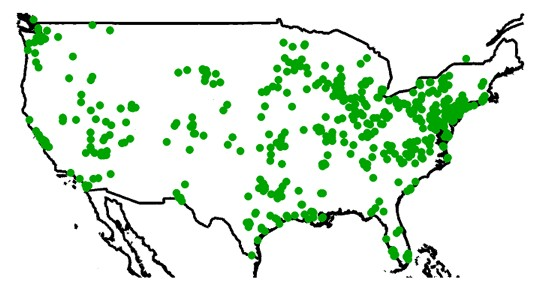
\includegraphics[width = 1\textwidth]{figures/localizationMap.jpg}
\label{fig:localizationMap}
\caption[Map of known webcam locations from the AMOS dataset.]{Many of the AMOS webcams are located in the United States, as shown in this map.}
\end{figure}


\section{Outline of the Paper}

We have many images from which we need to find interesting variants.  A lot of the variance is natural and controlled - day to night transitions, seasonal changes, and weather are all predictable and learnable.  First, we will present the mathematical tool Principal Component Analysis (PCA) as an algorithm to learn this natural variation.  Next, we will discuss different inputs to the PCA algorithm to best capture our goal.  Finally, we will show several visualization tools and evaluation criteria, and discuss their success in capturing interesting variation.



%
%\addtocontents{toc}{\newpage}
\chapter{Principal Component Analysis}
\label{cpt:pca}

Principal Component Analysis (PCA) is a powerful tool for 

\section{The PCA method}

Given a matrix $M$, we can use a linear algebra technique called singular value decomposition (SVD) to solve for matrices $U, S, V$ such that $M = U * S * V^T.$  For a given $k$ number of components


\begin{figure}[ht]
	\centering
	\subfigure[]{
		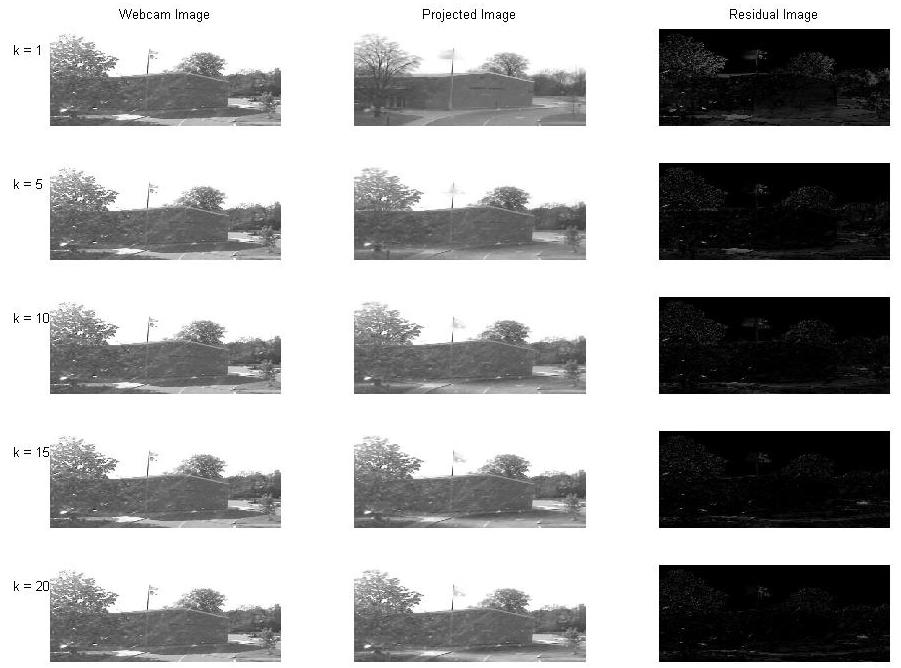
\includegraphics[width=1\textwidth]{figures/pcaIntroFigs.jpg}
	\label{fig:pcaIntroFigs}
	}
	\subfigure[]{
		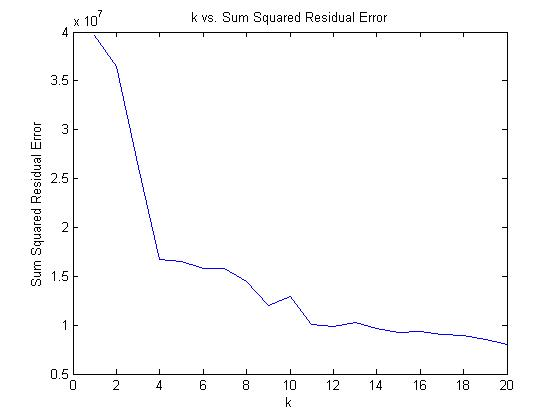
\includegraphics[width=.8\textwidth]{figures/pcaIntroPlot.jpg}
	\label{fig:pcaIntroPlot}
	}
		\caption[Learning a sky mask for a webcam scene.]{Figure \ref{fig:pcaIntroFigs} shows the first PCA component of a webcam scene.  By adding or subtracting this component, we control how dark or how light the sky is. Figure \ref{fig:pcaIntroPlot} shows that a simple thresholding of this image effectively segments the sky from the rest of the image.}
\end{figure}

\subsection{Incremental PCA}

In situations where dataset sizes conflict with memory constraints, we can use a modified algorithm called Incremental PCA.  Incremental PCA [reference to Matthew Brand]
\chapter{Visualization Tools}
\label{cpt:tools}

The main contribution of this project is automatic methods for visualizing how a webcam scene varies, and for understanding the most important variations.  In most natural scenes, we notice changes in lighting, weather, and camera conditions which are interesting, but fail to describe the typical behavior of a scene.  The goal of these tools is to learn these variations and to point out changes independent of them.  PCA is a commonly used tool, and
captures a linear model of consistent image variations.  By analyzing the results of certain PCA setups, we can obtain important and interesting information.

\section{Setup}

The most obvious way to learn about scenes is to take the PCA decomposition of the entire webcam scene.  Unfortunately, our data-set is too large for this to be feasible, so we must limit our inputs.  Instead of taking a random subset of the images, if we can intelligently limit the images we give, we can get better inputs.

\subsection{Temporal Narrowing}

The AMOS data-set consists mostly of outdoor scenes.  These outdoor scenes vary significantly over the course of a day, going from night to day and back.  The change in lighting dominates all other changes across the scene, and causes many images to be completely dark.  Instead of wasting 

\subsection{Sky Mask}
In many outdoor scenes, even when narrowed to a particular time of day, the most difficult image
variation to characterize is the sky.  PCA has a difficult time learning changes in sunlight, clouds,
and other characteristics of the sky, even among a set of images of one time of day.  The variance in the sky dominates the PCA reconstruction, causing it to ignore information that is more interesting in this context.

Fortunately, it is fairly easy to learn which regions of an image are most affected by this.  In practice, a side effect of the rising and setting of the sun is that the first principal component of most scenes is the sky, as shown in \ref{fig:2skyPCA}.  By thresholding the values of this vector, we can effectively segment the sky from the rest of the image, as shown in \ref{fig:2skyMask}.

This simple mask allows PCA to focus on more interesting changes in the image, and most of the results that follow use a simple mask to ignore the sky regions of the images.  By setting all pixels in the sky to 0, we can effectively remove this difficulty.


\begin{figure}[ht]
	\centering
	\subfigure[]{
		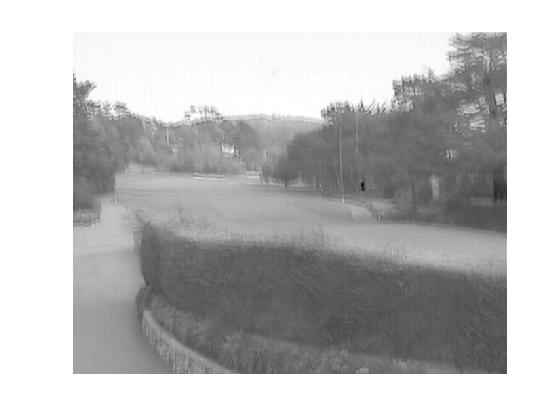
\includegraphics[width=0.45\textwidth]{figures/2skyPCA.jpg}
	\label{fig:2skyPCA}
	}
	\subfigure[]{
		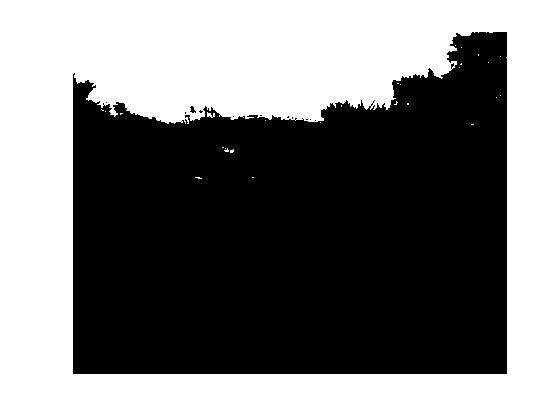
\includegraphics[width=0.45\textwidth]{figures/2skyMask.jpg}
	\label{fig:2skyMask}
	}
		\caption[Learning a sky mask for a webcam scene.]{Figure \ref{fig:2skyPCA} shows the first PCA component of a webcam scene.  By adding or subtracting this component, we control how dark or how light the sky is. Figure \ref{fig:2skyMask} shows that a simple thresholding of this image effectively segments the sky from the rest of the image.}
		
\end{figure}\subsection{Gradient Image}

\begin{figure}[ht]
	\centering
		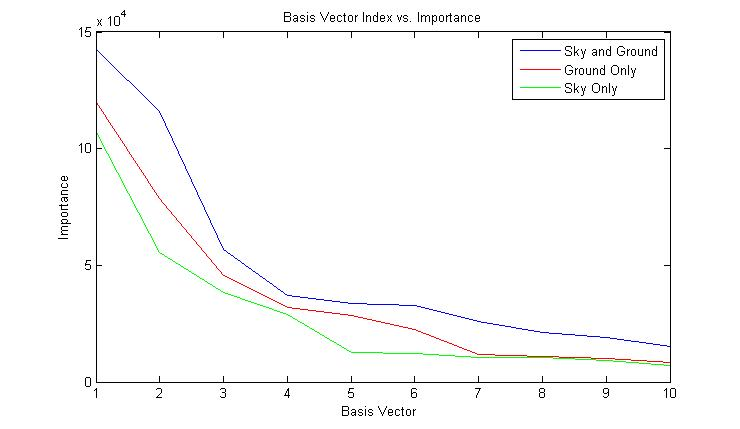
\includegraphics[width=1\textwidth]{figures/skyMaskFig.jpg}
	\label{fig:skyMaskFig}
	
		\caption[Sky Mask stuff.]{Figure \ref{fig:skyMaskFig} SOME STUFF.}
\end{figure}


Webcam images are very high-dimensional - a typical 320 x 240 gray scale image has 76,800 pixels, each of
which is a value from 0 to 255.  One way to simplify this space without changing the size of the image is to look at the gradient magnitude images of a scene.  

The x and y derivatives of an image are defined as $I_x(x,y) = I(x,y)-I(x-1,y)$ and $I_y(x,y) = I(x,y)-I(x,y-1)$ where the function $I(x,y)$ describes the intensities of an image's pixels.  Once we have calculated the derivative images, we define the gradient magnitude of an image to be $G(x,y) = I_x(x,y)^2 + I_y(x,y)^2$.

The gradient magnitude image highlights edges in an image, as they are image locations where pixel values differ greatly from their neighbors.  By performing PCA on the gradient magnitude images, we tend to ignore the potentially noisy surfaces of objects, and instead focus on the locations of the objects.  Figure \ref{fig:carsNoGradient} and Figure\ref{fig:carsGradient} show the edges of an interesting webcam image highlighted in a gradient magnitude image.


\begin{figure}[ht]
	\centering
	\subfigure[]{
		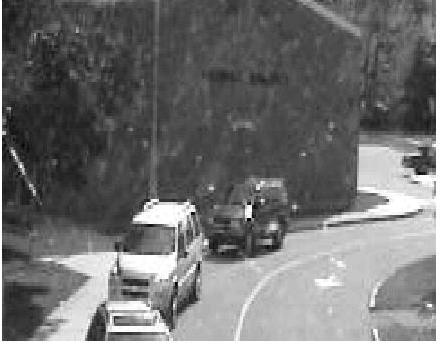
\includegraphics[width=0.45\textwidth]{figures/194cars.jpg}
	\label{fig:carsNoGradient}
	}
	\subfigure[]{
		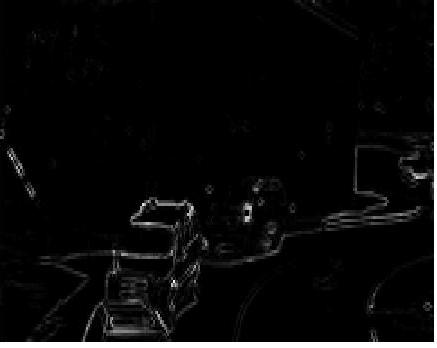
\includegraphics[width=0.45\textwidth]{figures/194carsGradient.jpg}
	\label{fig:carsGradient}
	}
		\caption[Focusing on object edges with gradient magnitude images.]{Figure \ref{fig:carsNoGradient} shows a grayscale webcam image. Figure \ref{fig:carsGradient} shows the gradient magnitude image of that frame.  Notice the noise is mostly removed and the edges are highlighted.}
\end{figure}

\section{Visualizations}

In this section, we present several tools to visualize the webcam scene based on criteria we will discuss in the next section.

\begin{figure}
	\centering
	\subfigure[]{
		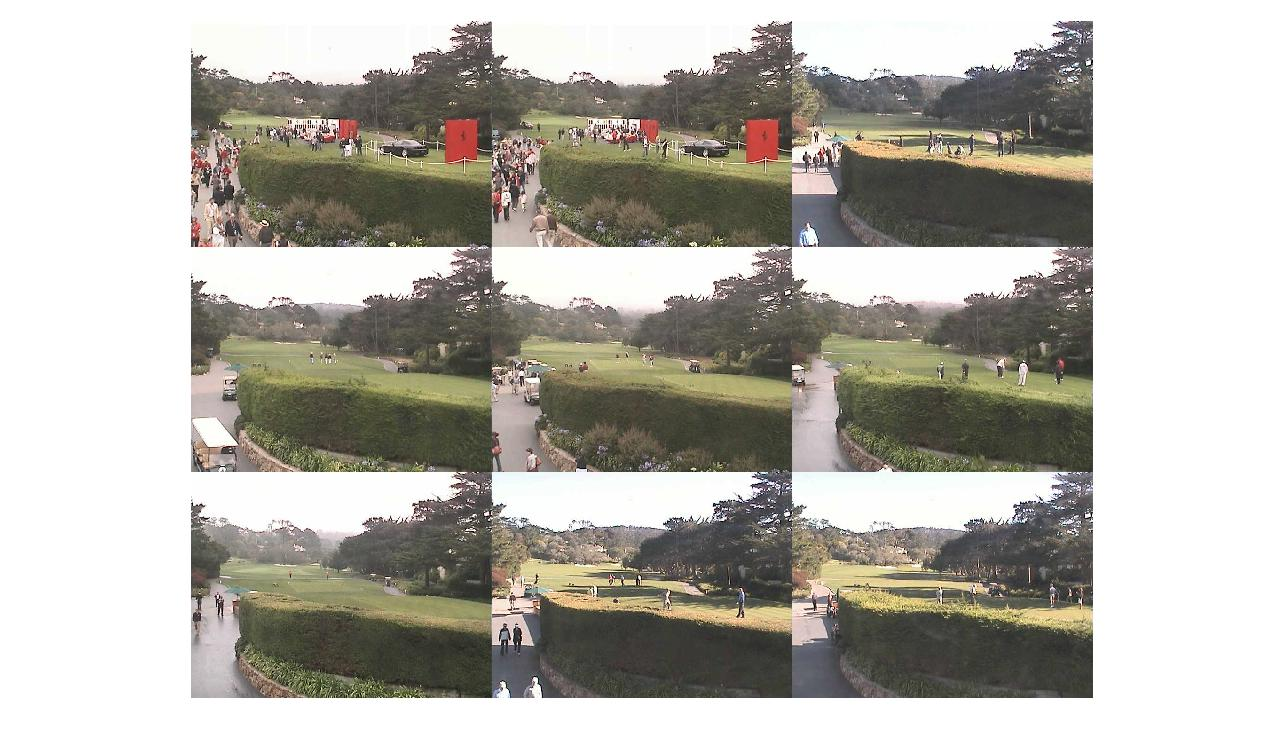
\includegraphics[width=1\textwidth]{figures/golfMontageNaive.jpg}
	\label{fig:golfMontageNaive}
	}
	\subfigure[]{
		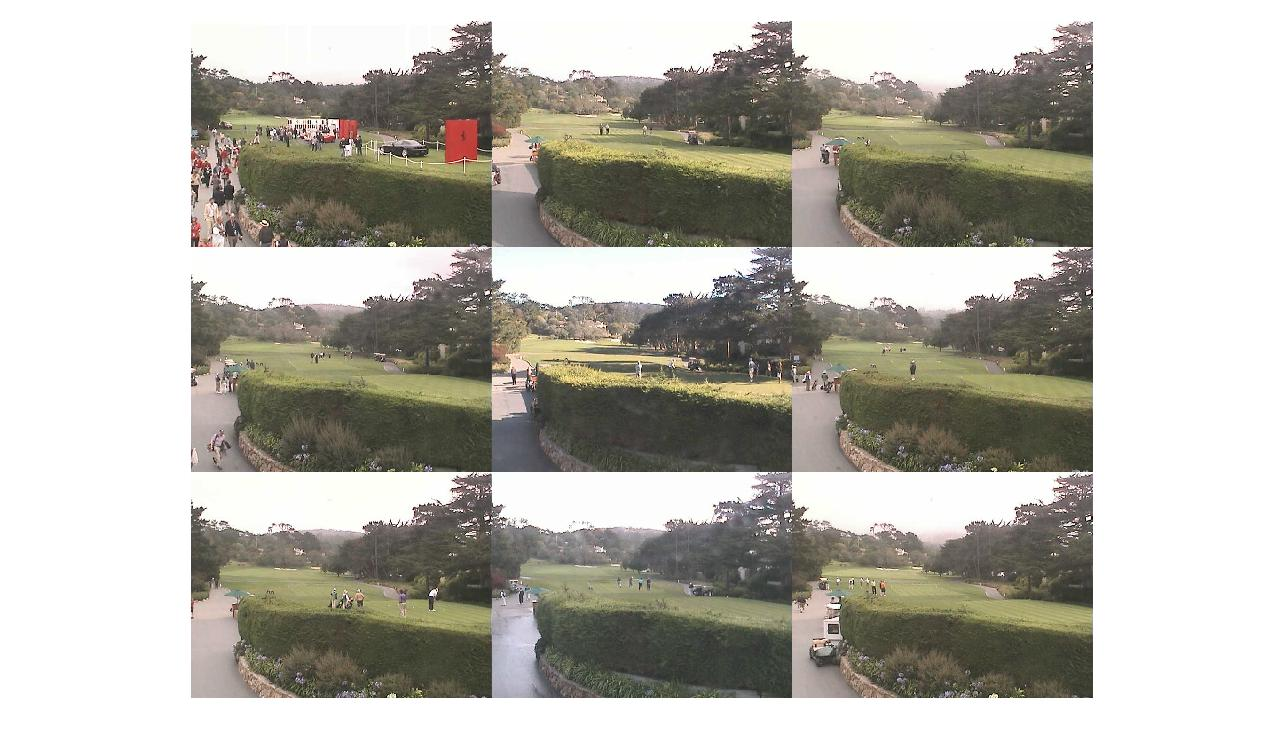
\includegraphics[width=1\textwidth]{figures/golfMontageSmart.jpg}
	\label{fig:golfMontageSmart}
	}
		\caption[Image montage techniques.]{Figure \ref{fig:golfMontageNaive} shows a montage of interesting images from a golf course webcam. Figure \ref{fig:golfMontageSmart} shows a montage of interesting images of the same scene, but attempts to omit similar images.}
\end{figure}

\subsection{Image Montage}

The simplest way to visualize a webcam scene is to view a montage of several images from that scene.  We can easily sort the images along some dimension, and then show the $n$ images with the highest values in that dimension.  Figure \ref{fig:golfMontageNaive} Is an example montage of several interesting images from a webcam scene.

\subsection{Well-Separated Set Montage}

In several of these montages, we notice that many of the most unusual images are similar to each other.  This presents the problem of finding unusual images that are different from the images we have already chosen.

A simple but effective algorithm for this problem uses the L2 norm in image space.  If we consider an image as a vector of pixel intensities, such as $v = \{v_1, ..., v_m\}$, the L2 norm of two images $v$ and $u$ is $$L2\_norm(v,u) = \sqrt{\sum_{i=1}^m{(v_i-u_i)^2}}$$  Given a large set of unusual images $\{x_1, ..., x_n\}$, we compute a distance matrix $D$ where $D_{i,j} = L2\_norm(x_i, x_j).$  Now we iteratively find unusual images by choosing the image that has the largest distance from all of the images we have chosen so far.  Specifically, for each remaining image calculate its distance to our set of exemplars, and choose the image whose distance is the smallest.  We define the distance of an image $x_0$ to a set of exemplars $\{x_1, ..., x_n\}$ as $$d = \min_i(D(x_0, x_i))$$In this way, on each iteration, we pick the image that is least likely to be similar to an image we have already selected.  We have found that a good way to seed this process is choosing the image with the highest unusualness score as our first exemplar.  \ref{fig:golfMontageSmart} shows how similar images are omitted by viewing results in this way.

\subsection{Two-dimensional Explorer}


Using a simple GUI, we can explore a webcam scene in two dimensions.  The GUI, shown in \ref{fig:2dGui}, displays a a plot of image scores for two different criteria, and displays the image corresponding to a mouseovered datapoint.  Using this GUI, it is possible to see which criterias are related and which are not, as well as makes it easier to learn how the criteria effects the scene. [I don't really know what to say in this section].

\begin{figure}[ht]
	\centering
		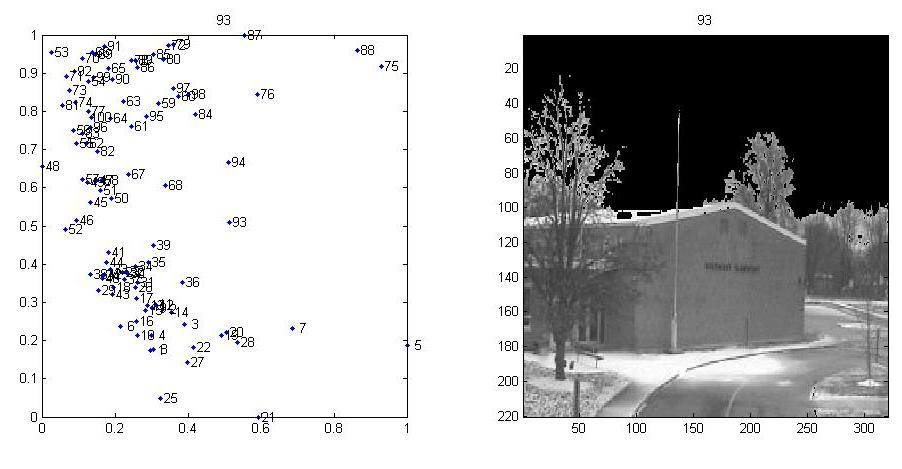
\includegraphics[width=1\textwidth]{figures/2dGui.jpg}
	\label{fig:2dGui}
	
		\caption[Exploring 2D image space using a simple GUI.]{Figure \ref{fig:2dGui} shows a webcam scene displayed using the 2D GUI.}
\end{figure}


\section{Characteristics of Image Residuals}

Once webcam scenes are projected onto a PCA basis, there are many different ways to analyze the results.  In this section, we will present several different criteria for evaluating this appearance model of a scene, the meaning behind each criteria, and results.

[I don't love the term criteria, but I think it encapsulates the idea of this section...]

\subsection{PCA coefficient vector magnitude}

\begin{figure}
	\centering
	\subfigure[]{
		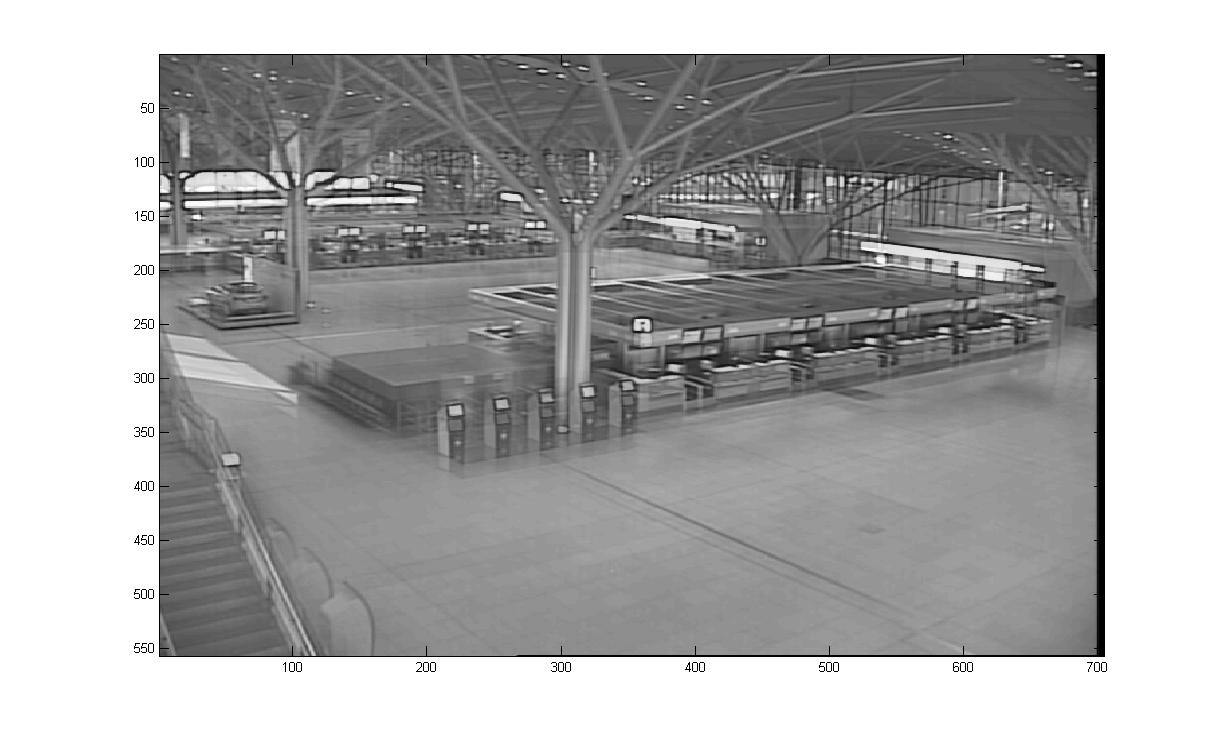
\includegraphics[width=.8\textwidth]{figures/vectorMagnitudeMean.jpg}
	\label{fig:vectorMagnitudeMean}
	}
	\subfigure[]{
		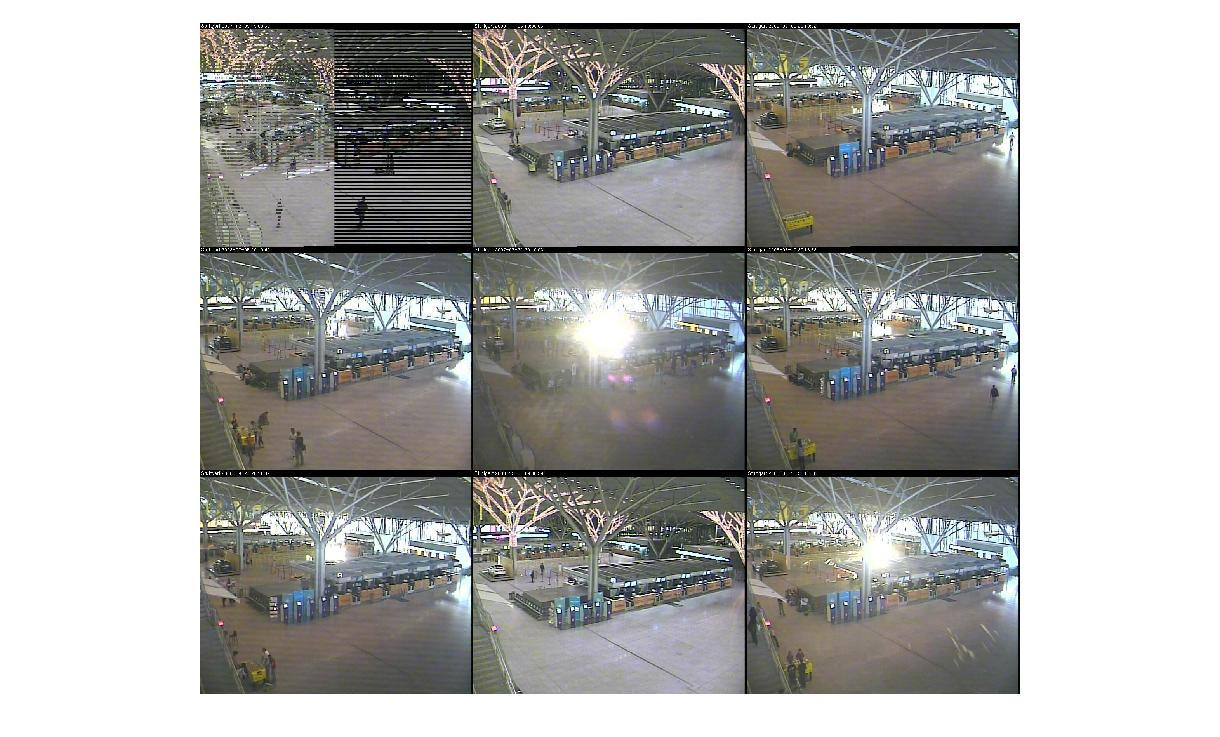
\includegraphics[width=1\textwidth]{figures/vectorMagnitudeMontage.jpg}
	\label{fig:vectorMagnitudeMontage}
	}
		\caption[Criteria: Gradient Magnitude.]{Figure \ref{fig:vectorMagnitudeMean} shows the mean image of an airport webcam scene. Figure \ref{fig:vectorMagnitudeMontage} shows several images found using this technique that are far from the mean.}
\end{figure}

For each image in a scene, PCA gives a vector of coefficients that correspond to the best linear combination of basis images to reconstruct that image.  From this vector, we can assign each image a score equal to the magnitude of this vector.  For a vector $v = (v_0, v_1, ..., v_n)$, the vector magnitude is $$||v||=\sqrt{\sum_{i=0}^nv_i^2}$$This effectively gives us a measure for how far from the mean image in our basis space each image is.  Figure \ref{fig:vectorMagnitudeMean} shows the mean image of a webcam scene and Figure \ref{fig:vectorMagnitudeMontage} shows several images from that webcam scene that are especially far from the mean.



\subsection{Residual Error}

Given an image and a PCA basis, we can project the image onto the basis and see how well we can reconstruct the image.

\begin{figure}
	\centering
		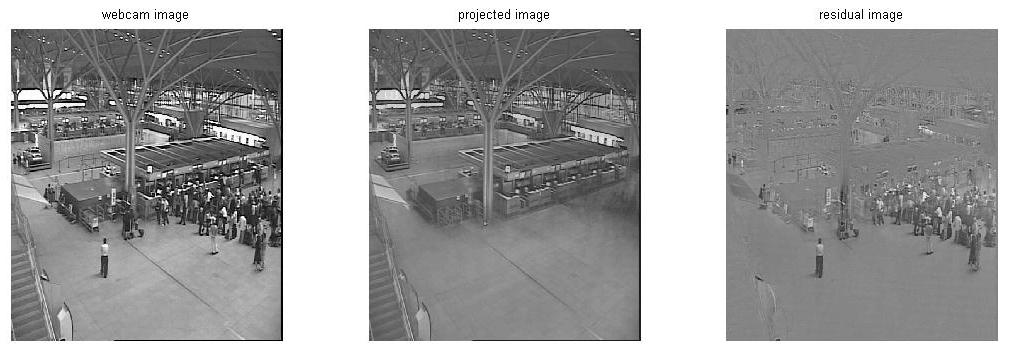
\includegraphics[width=1\textwidth]{figures/residualReconstruction.jpg}
	\label{fig:residualReconstruction}
	
		\caption[Residual Reconstruction.]{Figure \ref{fig:2dGui} show a webcam scene image, the reconstruction of that image from a PCA basis, and the residual image.}
\end{figure}

[Figure of subplot with image, reconstruction, and residual]

\begin{figure}
	\centering
		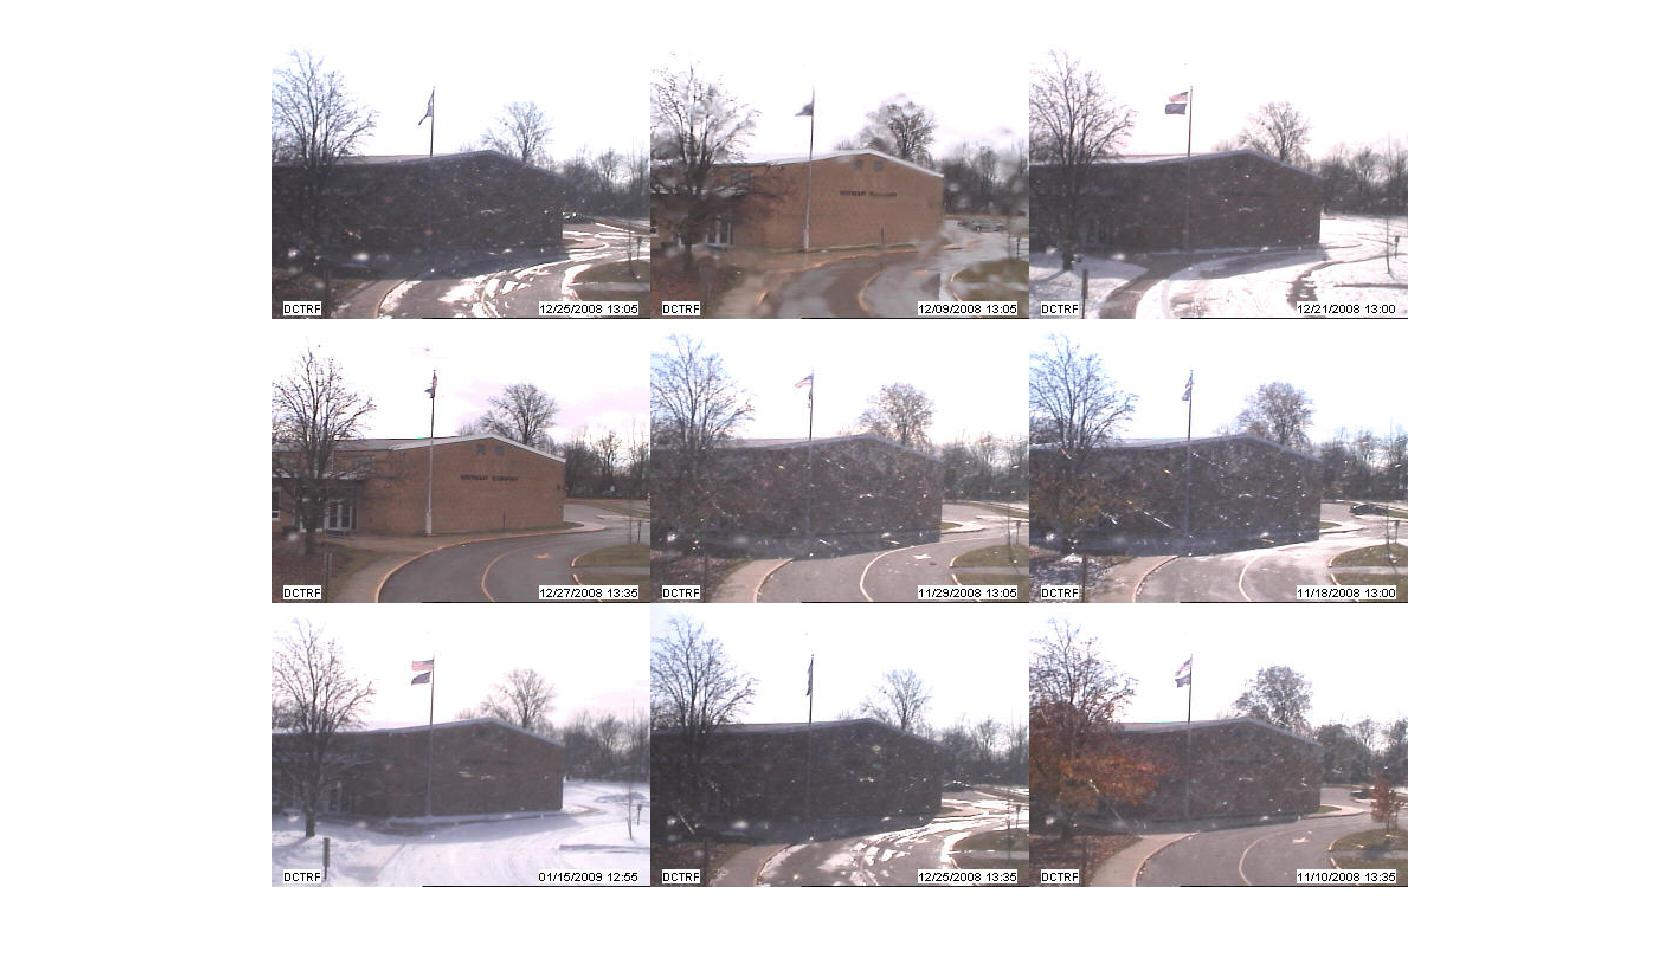
\includegraphics[width=1\textwidth]{figures/residualSSDmontage.jpg}
	\label{fig:residualSSDmontage}
	
		\caption[Residual SSD Montage.]{Figure \ref{fig:residualSSDmontage} show a webcam scene image, the reconstruction of that image from a PCA basis, and the residual image.}
\end{figure}

[figure of montage sorted be residualSSD, showing some noisy images and some with real foreground objects]


\subsection{Variance Model}

We can estimate the variance image of a webcam scene as the average of the square of each residual image.  This image gives a good summary as to where most activity occurs in a webcam scene.  Several examples are shown in Figure \ref{fig:severalVarianceImages}.

\begin{figure}
	\centering
		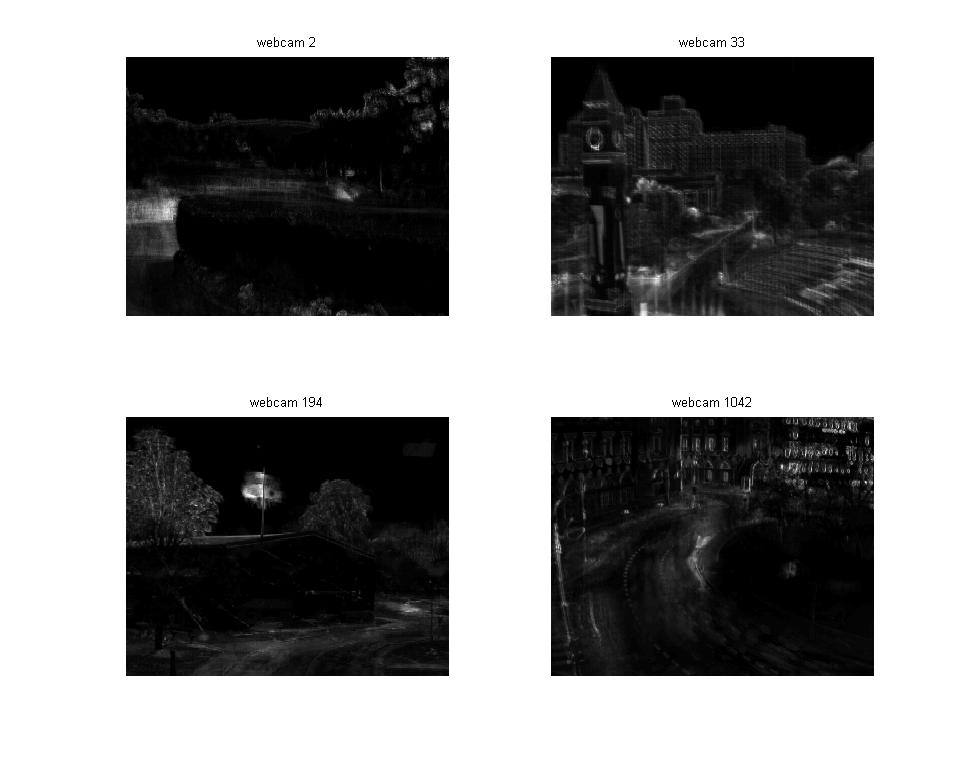
\includegraphics[width=1\textwidth]{figures/severalVarianceImages.jpg}
	\label{fig:severalVarianceImages}
	
		\caption[Several variance images.]{Figure \ref{fig:severalVarianceImages} shows estimated variance images from several webcam scenes.}
\end{figure}

One we have this variance image, we can attempt to isolate independent pixels in a z-score image.  We define our z-score image as $$Z(x,y) = \frac{R(x,y)} { V(x,y)}$$ where $R(x,y)$ is the residual value of the pixel and $V(x,y)$ is the variance value of the pixel.  By summing the per pixel z-score for an particular image, we can infer how atypical the residual of that image is.  Figure \ref{fig:residualZScoreMontage} shows several images that contain atypical objects.  Such a tool can be used to quickly highlight unusual behavior in a scene.

\begin{figure}
	\centering
		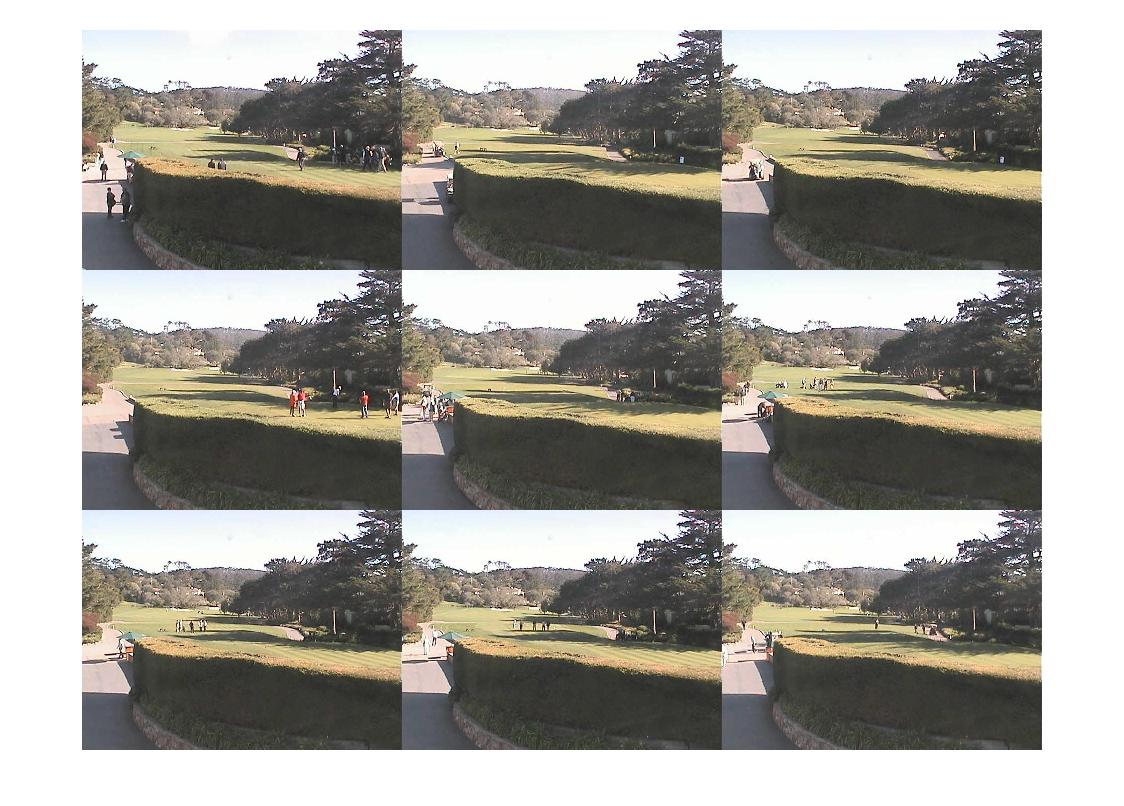
\includegraphics[width=1\textwidth]{figures/residualZScoreMontage.jpg}
	\label{fig:residualZScoreMontage}
	
		\caption[Z-Score Montage.]{Figure \ref{fig:residualZScoreMontage} shows several images from the same scene as \ref{fig:residualSSDmontage}, but with more atypical objects.}
\end{figure}





\subsection{Statistical Distribution of Residual Images}

We can also try to learn about an image reconstruction by treating its residual image as samples from an 
underlying probability density function.  If image deviations are due mostly to noise, we predict that these deviations will be normally distributed, but as shown in \ref{fig:severalHists}, this is not always the case.  We have found that these distributions vary in the same way as webcam scenes, and analyzing them in the right way tells an interesting story.


\begin{figure}
	\centering
		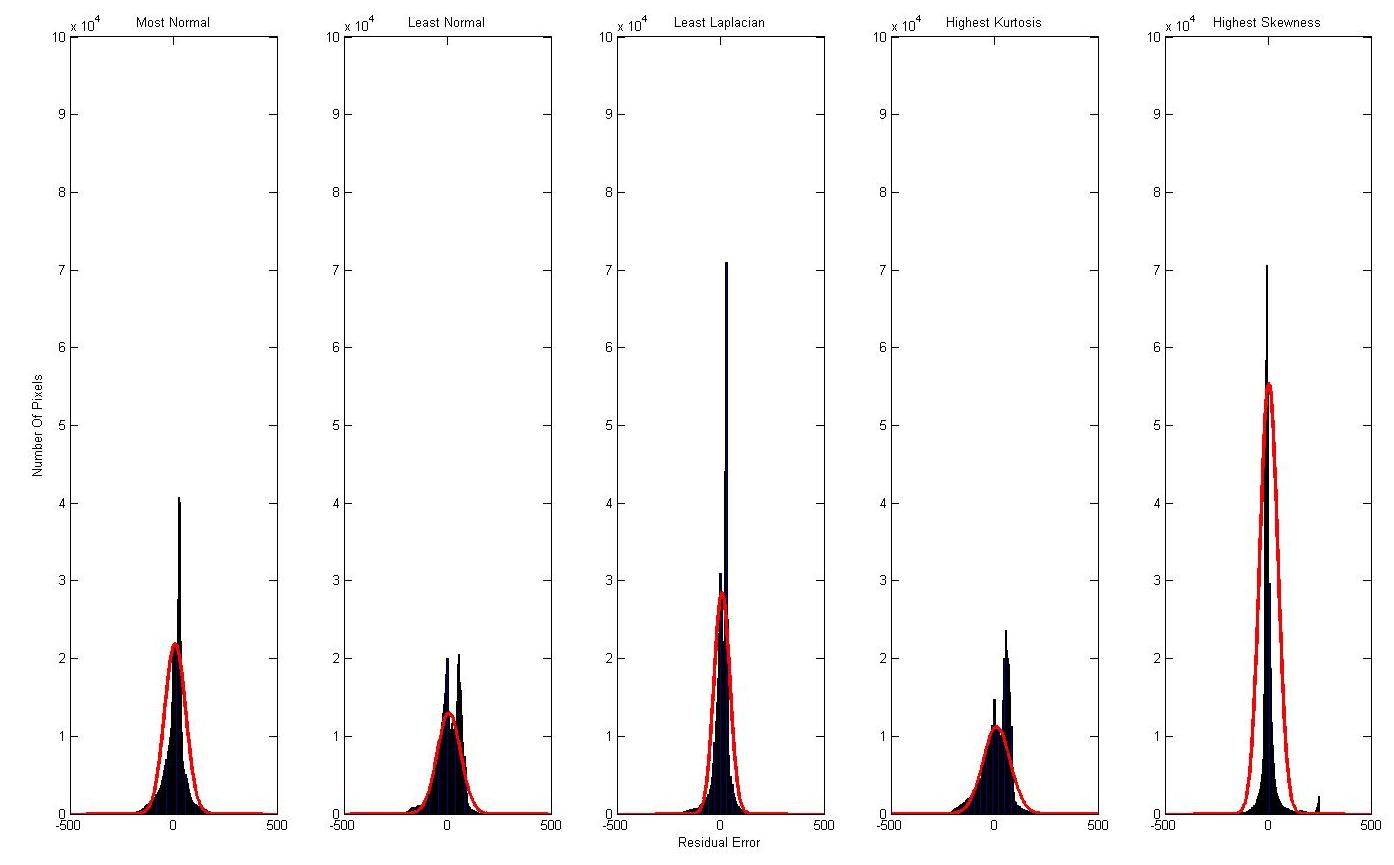
\includegraphics[width=1\textwidth]{figures/severalHists2.jpg}
	\label{fig:severalHists}
	
		\caption[Several residual image histograms.]{Several residual image histograms and the the best approximation of a normal distribution fitting the data.}
\end{figure}



\begin{figure}
	\centering
	\subfigure[]{
		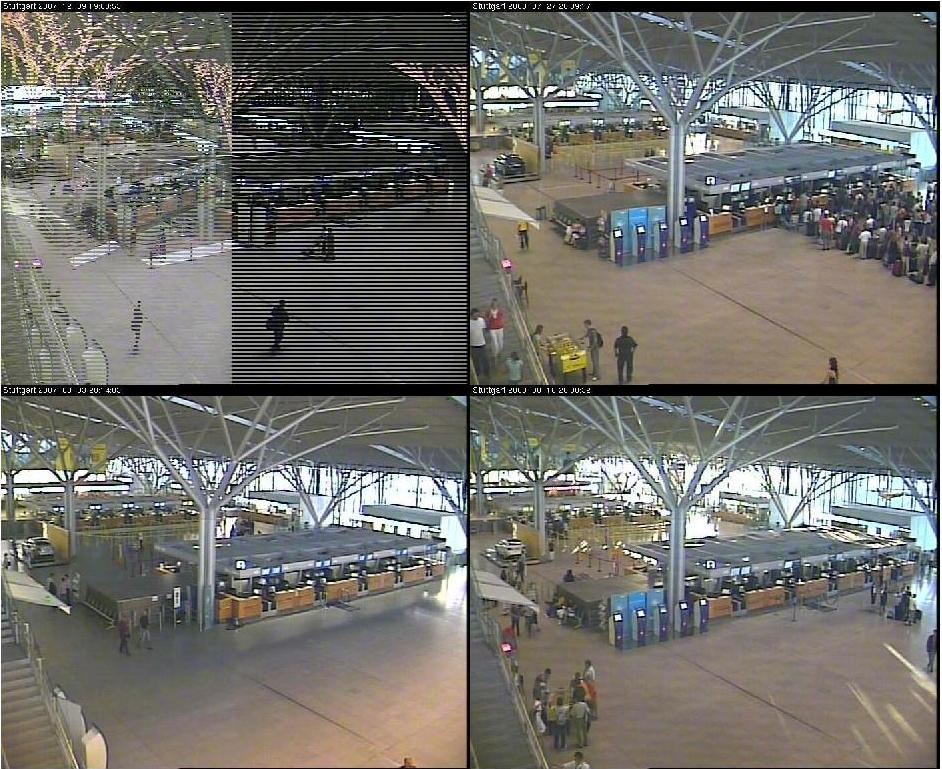
\includegraphics[width=.6\textwidth]{figures/leastNormal.jpg}
	\label{fig:leastNormal}
	}
	
	\subfigure[]{
		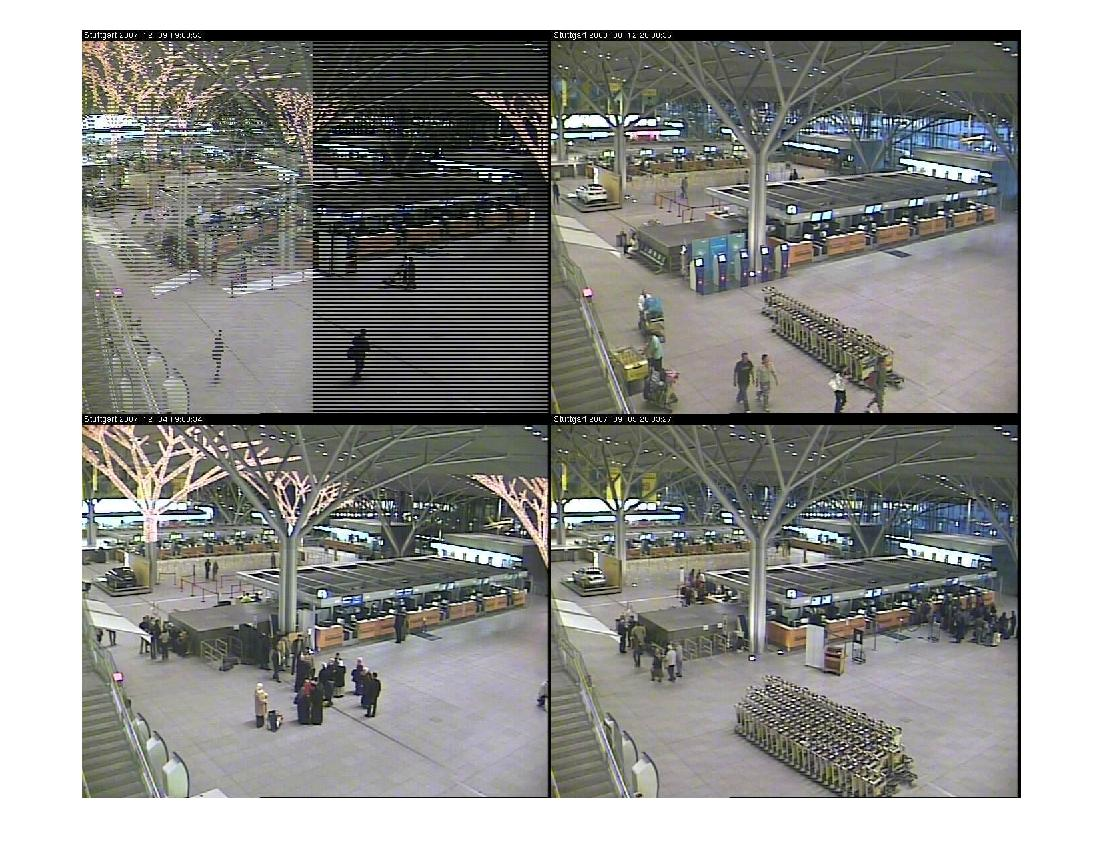
\includegraphics[width=.6\textwidth]{figures/leastLaplacian.jpg}
	\label{fig:leastLaplacian}
	}
	
			\caption[Least Gaussian and Least Laplacian Images.]{Figure \ref{fig:leastNormal} shows a montage of interesting images from an airport scene that were labeled very non-guassian. Figure \ref{fig:leastLaplacian} shows a montage of interesting images from an airport scene that were labeled very non-laplacian.}
\end{figure}



\begin{enumerate}
\item{\textbf{Gaussian Likelihood}}

The most obvious way to do this is to treat each residual image pixel as a sample from a normal distribution.  We can easily estimate the mean and variance of this PDF and then, for each residual value, use the normal distribution equation 

$$f(x|\mu,\sigma)=\frac{1}{\sigma\sqrt{2\pi}}e^{\frac{(x-\mu)^2}{2\sigma^2}}$$

 


\item{\textbf{Laplacian Likelihood}}

Many of the residual images have a majority of pixels that are very close zero.  This causes the histogram to look very similar to a laplacian distribution.

$$f(x|\mu,\beta)=\frac{1}{2\beta}e^{\frac{-|x-\mu|}{\beta}}$$

\item{\textbf{Kurtosis}}

The kurtosis of a real-valued random variable is a measure of its peakedness.  Larger values of kurtosis means more variance is due to less frequent extreme deviations rather than frequent less extreme deviations.  It is defined as $$\gamma_2=\frac{\mu_4}{\sigma^4}$$ where $\mu_4$ is the fourth moment about the mean and $\sigma^4$ is the estimated standard deviation to the fourth power.  For a function $f(x)$, the $k^{th}$ moment about the mean is defined as 

$$\mu_k = \int_{-\infty}^{\infty}{(x-\mu)^kf(x)dx}$$

We can use this measure 

\item{\textbf{Skewness}}

The skewness of a random variable is a measure of asymmetry.  Higher skewness values mean deviations on one side of the mean do not have corresponding deviations on the other side.  It is defined as $$\gamma_1=\frac{\mu_3}{\sigma^3}$$ where $\mu_3$ is the third moment about the mean and $\sigma^3$ is the cube of the standard deviation.

This measure can be used


\end{enumerate}




\appendix                        % now we start appendicies
\chapter{The English Language and Other Confusing Things}
\label{app:english-language}

While this guide answers most questions about how to format a thesis, it does
not address questions about English grammar, use of abbreviations, punctuation,
spelling, and other confusing subjects.  Students should obtain a dictionary
and a style of grammar book to refer to as questions arise.  The dictionary is
important because most electronic spelling checkers are not complete and do not
contain definitions.  (You may also need to refer to some of the references you
cite for the spelling of technical terms.)  The grammar or style book is useful
for checking grammar and punctuation rules.  A good style manual contains
information about correct English usage as well as advice for preparing a
manuscript.  \textit{A Manual for Writers of Term Paper, Theses, and
Dissertations}~\cite{Turabian} is one such concise and inexpensive manual based
on the lengthy and more expensive \textit{Chicago Manual of
Style}~\cite{ChicagoManual}.  

The following rules will help you avoid three mistakes frequently made
by students:
\begin{itemize} 
 \item Hyphenated words must begin and end on the same page.

 \item When a page break falls in the middle of a paragraph, at least
two lines of text from that paragraph must appear on the second page.

 \item At least one line of text from a section or subsection must
appear on the same page as the title of that section or subsection.
\end{itemize}

%%% Local Variables: 
%%% mode: latex
%%% TeX-master: "thesis-main"
%%% End: 

\chapter{Procedures and Deadlines}
\label{app:procedures}

\paragraph{Deadlines}
At least one semester prior to the semester in which you believe you will
complete all requirements for your degree, please be sure to consult with your
department's graduate administrative assistant or coordinator to be sure you
are aware of all requirements and deadlines with regards to your thesis and the
submission of your thesis.  Deadlines are printed in the course listings
schedule book and are posted online.  If you cannot make certain deadlines, you
may have to postpone your graduation accordingly.  M.S.\ and D.Sc.\ students
have a special deadline by which they must submit an initial draft of their
thesis so that it can be reviewed for formatting, to make sure it conforms to
the essential formatting requirements, as illustrated in this sample guide.
Ph.D.\ students must follow the requirements of the Office of Graduate Students
in Arts and Sciences (GSAS).  The GSAS office does not have an special
formatting deadlines, but you should still contact that office if you have
questions about your formatting.

\paragraph{Oral Examination}
Each member of the oral examining committee must be given a copy of the thesis
or dissertation, in final form, in sufficient time to study it before the oral
examination.  Members of the examining committee have the right to request
rescheduling of the examination if these copies are not made available to them
at least one week in advance of the scheduled examination date.  Copier paper
may be used for these preliminary copies.

\paragraph{Final Copies}
After the oral defense, final copies of the thesis or dissertation approved by
the examination committee and department are to be distributed as follows, on
or before the date stated in the current academic calendar.  All final copies
must be printed using only one side on high-quality (either watermarked or
specifying as having 10-25\% cotton), 8.5 x 11 inch white paper, and minimum
20-pound weight.  Students should submit their final materials to the office(s)
listed in the first item below, plus all other materials itemized below should
be submitted accordingly, if needed:
\begin{itemize}
  \item \uline{Four copies of the thesis or dissertation need to be submitted
	  as follows:} Each should be placed in a separate manila envelope with
	  a copy of the title page securely attached.  One of these two will be
	  retained in the Washington University library; another will be sent
	  back to you after being professionally bound;  the other two copies
	  are for your advisor and department.  Two copies (along with the
	  following listed materials) get delivered to Engineering Student
	  Services.  Two copies get delivered to your department (also with the
	  short title page included as listed immediately below---although,
	  none of the other additional items listed further below are needed
	  for the department copies).  \textbf{NOTE FOR PH.D.\ STUDENTS:}  All
	  four copies get delivered to the GSAS Office.  See GSAS dissertation
	  guidelines from their web site.
        
  \item \uline{a loose sheet containing} (1) a \uline{short title} of 35
	  letters or less (including spaces), (2) the author's last name, (3)
	  the degree, and (4) the year of its award, centered on the page and
	  punctuated as in the example.\footnote{See the sample short title
	  page for this document} This short title sheet is to be placed at end
	  of your thesis/dissertation.
	
  \item one \uline{extra} loose copy of the abstract (this applies to doctoral
	  students only), \uline{double spaced}, for publication in
	  Dissertation Abstracts. 
  
  \item one \uline{extra} loose copy of the \uline{title page} (this applies to
	  doctoral students only) for the microfilming contract.

  \item the \uline{original \textbf{and} a photocopy of the University
	  Microfilms Inc.\ publishing agree\-ment contract} (this applies to
	  doctoral students only).  This contract is available from the
	  Engineering Student Services web site.  If a registration to your
	  claim to copyright is desired, attach a certified check, cashier's
	  check, or money order for the current price listed in the University
	  Microfilms contract.  Personal checks are not accepted.  The
	  microfilming contracts are available in Lopata 324.  The check or
	  money order should not have an expiration date.
\end{itemize}

Four copies in all are to be submitted, as per details listed above.  See the
first bulleted item for full details.  Please follow instructions carefully.
Contact Engineering Student Services if you have questions.  Ph.D.\ students
may contact the Graduate School of Arts and Sciences.

%%% Local Variables: 
%%% mode: latex
%%% TeX-master: "thesis-main"
%%% End: 

\chapter{Thesis Format Checklist}

\newcommand{\smallblank}{\underline{\hspace{0.25in}}\,}
\newcommand{\largeblank}{\underline{\hspace{0.75in}}\,}

{\footnotesize \textbf{NOTE: If you have significantly varied formatting from that
which is shown in this document, please complete this form and submit it to
Engineering Student Servcies when you submit your thesis for format review.}}

Author's Name:  \underline{\hspace{4.0in}} \\
Title page font:  \smallblank 12 point \indent \smallblank 14 point \\
Table of contents chapter titled font: \smallblank plain \indent \smallblank bold \\
First level table of contents indentation (0 to 0.5 inch): \largeblank \\  
Second level table of contents indentation (0 to 1 inch): \largeblank \\
Body text font: \smallblank 10 point \quad \smallblank 11 point \quad \smallblank 12 point \\
Body text line spacing: \smallblank 1.5 \quad \smallblank 2 \indent \\
Body text justification: \smallblank left \quad \smallblank full \\
Paragraph indentation (0 to 0.5 inch):  \largeblank \\
Chapter title position (1.5 to 3 inches below top edge):  \largeblank \\
\begin{tabular}{@{}lll}
Chapter title style: \smallblank with word ``Chapter'' & \multicolumn{2}{l}{\smallblank without word ``Chapter''} \\
Chapter title:  \smallblank (10 to 36 point) & \smallblank plain & \smallblank bold \\
& \smallblank centered & \smallblank left justified \\
Section heading: \smallblank (10 to 24 point) & \smallblank plain & \smallblank bold \\
& \smallblank centered & \smallblank left justified \\
Subsection heading:  \smallblank (10 to 18 point) & \smallblank plain & \smallblank bold \\
& \smallblank centered & \smallblank left justified \\
Unnumbered heading: \smallblank (10 to 14 point) & \smallblank plain & \smallblank bold \\
& \smallblank centered & \smallblank left justified
\end{tabular} \\
Label tables as: \smallblank Table \quad \smallblank Figure \\
Reference list style (parenthetical, etc.): \underline{\hspace{3.0in}}

%%% Local Variables: 
%%% mode: plain-tex
%%% TeX-master: t
%%% End: 

\wrappedappendix{Special Notes for \LaTeX{} Users, Including a \\
	\hbox to 1.0in{}Demonstration of Wrapping Appendix Titles}
{Special Notes for \LaTeX{} Users, Including a Demonstration of Wrapping Appendix Titles}
%\chapter{Special Notes for \LaTeX{} Users}
\label{app:latex-notes}

\newcommand{\cmd}[1]{\texttt{$\backslash$#1}}

It is strongly recommended that you use this file as a template for your
thesis, since it greatly simplifies conforming to the required formatting
standards.

There are several important points that students using the \LaTeX{} version of
this template should verify before submitting a thesis.

\section{Front Matter}

Much of the front matter (i.e., the Roman numbered pages) is automatically
generated.  Use \cmd{renewcommand} command to customize the fields of these
templates.  For example,
\texttt{\cmd{renewcommand}$\{$\cmd{thesisauthor}$\}\{$your name here$\}$} will
customize the author name.

\sloppy
Most authors will need to customize the \cmd{thesismonth}, \cmd{thesisyear},
\cmd{thesisauthor}, \cmd{thesisauthorlastname}, \cmd{thesisdefensedate},
\cmd{thesistitle}, \cmd{thesisshorttitle}, \cmd{thesisdepartment},
\cmd{thesisfield}, \cmd{thesissupervisor}, and \cmd{thesiscommittee}
fields.  Examples of these can be seen in the sample \texttt{thesis-main.tex}
file.

\fussy
You must also specify \texttt{phdthesis}, \texttt{dscthesis}, or
\texttt{mastersthesis} when selecting the \cmd{documentclass}.  An
example can also be seen in the sample \texttt{thesis-main.tex} file.

\section{Table of Contents and Bibliography}

The Table of Contents is automatically generated.  \texttt{latex} should be run
twice in succession after making any changes to the Table of Contents.

Due to the way \LaTeX{} formats the Table of Contents, long appendix titles
will not automatically wrap and indent properly.  If you need to use a long
appendix title, you must manually wrap and indent the appendix's
table-of-contents entry.  The \cmd{wrappedappendix} command is defined in this
template to assist with this; an example is seen at the top of the sample
\texttt{thesis-appendixD.tex}.  This requirement only applies to appendix
titles: other section titles will automatically wrap properly, including
entries in the List of Tables and List of Figures.

If changes need to be made to the Table of Contents' formatting, you can use
the \cmd{addtocontents} command to insert some formatting commands
directly into the Table of Contents page.  More significant changes can be made
by editing the \texttt{.toc} file that \LaTeX{} automatically generates.
However, editing this file by hand is not recommended unless absolutely
necessary, since it will automatically be re-generated the next time \LaTeX{}
is run.

Like the Table of Contents, the Bibliography is automatically generated.  After
editing the bibliography file, you should run \texttt{latex}; run
\texttt{bibtex}; and re-run \texttt{latex} twice in succession.

\section{Captions}

\sloppypar
Multiline captions will not automatically be centered.  To correct this, place
\cmd{usepackage[center]$\{$caption$\}$} in the document preamble.  The sample
\texttt{thesis-} \texttt{main.tex} already includes this command.

\section{Widows and Page Breaks}

\LaTeX{} may create widows if you have a paragraph followed by a list.  To get
rid of this widow, you must force \LaTeX{} to break the page somewhere else.
Either insert a \cmd{newpage} command before the paragraph, or insert a
\cmd{samepage} command between the paragraph and the list.

\LaTeX{} may also create widows in the Tables of Contents.  You can force
\LaTeX{} to break the page in a more convenient location by inserting
\cmd{addtocontents$\{$toc$\}\{$\cmd{newpage}$\}$} before the corresponding
\cmd{chapter}, \cmd{section}, \cmd{subsection}, or \cmd{subsubsection} command
in the text.

Excluding these two situations, \LaTeX{} should not create orphans or widows.
However, in some situations it may place page breaks at strange places --- such
as several inches above the bottom margin --- in order to avoid creating
orphans or widows.  You can fix this by altering the \cmd{clubpenalty} or
\cmd{widowpenalty}, or by manually adding \cmd{newpage}s where \LaTeX{} guesses
incorrectly.


% A good place for the bibliography.
%
\bibliographystyle{plain}
\begin{spacing}{1.0}
\bibliography{./thesis-references}
\end{spacing}
\nocite{*}
%
% The Vita should be the last thing
%
%\begin{thesisauthorvita}
%
% This is just a sample of what to do in a vita
%
%%
%
% Sample  Vita
% This is done in a list environment.
%
% Personal heading
\begin{center}
{\large\thesisauthor}
\end{center}
%
% Need to 'fold' long labels
%
\newcommand{\vitalabel}[1]%
  {\raisebox{0pt}[1ex][0pt]
    {\makebox[\labelwidth][l]%
      {\parbox[t]{\labelwidth}{\hspace{0pt}\textbf{#1}}}}}
%
% Here's the list definition
%
\begin{list}
  {}%                                        nodefault label
  { \renewcommand{\makelabel}{\vitalabel}%   setting labels
    \setlength{\labelwidth}{100pt}%          label width
    \setlength{\leftmargin}{120pt}%
    \setlength{\itemindent}{0pt}%            don't indent first line of items
    \setlength{\parsep}{\baselineskip}%               space between paragraphs
    \setlength{\itemsep}{5pt}%               additional space between items
    }
\item[Date of Birth] July 28, 1965
\item[Place of Birth] Saint Paul, Minnesota
\item[Degrees] B.S.\ Magna Cum Laude, computer Science, May 1988 \\
	M.S.\ Computer Science, December 1990 \\
	D.Sc.\ (or Ph.D.) Some Department, May 2007
\item[Professional\linebreak Societies]
  Association for Computing Machines \\
  The Touring Society \\
  The Free Software Foundation
\item[Publications]
  Student, I.\ D.\ (2005).\ \LaTeX{} document class for Sever Institute,
  \textit{The \LaTeX{} J.} \textbf{10}(4):~323--336.
  
  Student, I.\ D.\ (2005).\ More \LaTeX{} wisdom, \textit{Another \LaTeX{} J}.
  \textbf{42}(7):~100--101.
\end{list}
\flushright
\thesismonth\ \thesisyear


%\end{thesisauthorvita}

\flushleft

\begin{thesisshorttitlepage}
\end{thesisshorttitlepage}

%%% Local Variables: 
%%% mode: latex
%%% TeX-master: "thesis-main"
%%% End: 


\end{document}
